\section{Experimental analysis}

In this section, we evaluate the experimental results of
the proposed exact-join and approximate-join algorithms. 

 We will compare
their effectiveness on the following datasets from different
application scenarios in Java $1.6.0$ and run on a
Windows XP with dual-core Intel Xeon CPU 4.0GHz, 2GB RAM, and a 320GB hard disk.


\subsection{Datasets}


To evaluate the impact of taxonomy information on classification performance, we generated taxonomies over each dataset.
While aggregation trees on continuous attributes have been generated by applying discretization procedures, aggregation trees
on nominal attributes are analyst-provided. Note that, in real-life contexts, aggregation trees may be semi-automatically derived, for instance, from lexical or geographical databases (e.g., the WordNet Lexical Database [18]). A more detailed description of the
applied multiple-taxonomies follows.


We use three datasets: US addresses (\textbf{USPS}),
conference titles  (\textbf{CONF}), and gene/protein data
(\textbf{SPROT}). These datasets differ from each other in terms of rule-number, rule-complexity, data-size and string-length. Our goal in choosing these diverse sources is to understand the usefulness of algorithms in different real world environments.

\smallskip
\noindent \textbf{{USPS}}: We downloaded common person names, street names,
city names, states, and zip codes from the United States Postal
Service website ({\footnotesize http://www.usps.com}). We then generated
one million records, each of which contains a person name, a street
name, a city name, a state, and a zip code. USPS also publishes
extensive information about the format of US addresses, from which we
obtained 284 synonym pairs. The synonym pairs covers a wide range of alternate
representations of common strings, e.g. street $\rightarrow$ st.


\noindent \textbf{{CONF}}: We collected 10,000 conference names
from more than ten domains, including Medicine and Computer
Science.
We obtained $1000$ synonym pairs between the full names of conferences and their
abbreviations by manually examining conference websites or homepages
of scientists.


\noindent \textbf{{SPROT}}: We obtained one million gene/protein records
from the Expasy website ({\footnotesize http://www.expasy.ch/sprot}).
Each record contains an identifier (ID) and its name.
%For example, the two records, \textit{(O00203, Adapter-related protein complex 3
%beta-1 subunit)} and \textit{(O00203, AP-3 complex subunit
%beta-1)}, refer to the same gene as they have the same ID.
In this dataset, each ID has $5\sim22$ synonyms. We generated 10,000 synonym rules describing gene/protein
equivalent expressions.

In each dataset we subtracted from the scores their minimum,
so that the smallest score is 0, without affecting the
ordering. The minimum is then added back at query time.




\begin{figure}
  \small
  \centering
  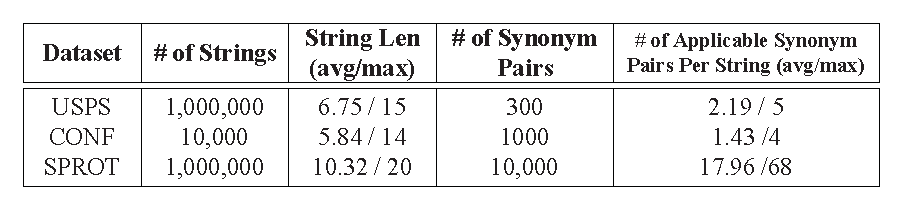
\includegraphics[width=\linewidth]{figures/Characteristics_Datasets}
   \vspace{-6mm}
  \caption{Characteristics of Datasets.}
  \label{tab:data_characteristics}
\end{figure}


Figure~\ref{tab:data_characteristics} gives the characteristics of the
three datasets.
